\section{Method}
\label{sec:method}

In this section, we develop our method for reasoning about movement within a coarse `unit cube' space.
We start from trace data of positions, identify how this trace data is transformed into occupied boxes as well as nodes in a graph, then discuss properties of one thing moving in space, then move to multiple things moving in space.

\subsection{Foundations and Definitions}
We begin with a trace $T$ of spatial data, containing a time sequence of $xyz$ positions.
We call the thing that is moving an \eb{actor}, designated by $\bigstar$.
Each element in trace $T$ occurs at a time $t$.
Let there exist a space $\cube^3 \equiv \mathbb{Z}^3$ called ``cube 3", and a function $f_{\cube}: \bigstar_i (x,y,z) \in \mathbb{R} \rightarrow (a,b,c) \in \mathbb{Z}$, such that:

$$f_{\cube}(x,y,z) = (\lfloor x \rfloor, \lfloor y \rfloor , \lfloor z \rfloor )$$

Let the $i$th element of the trace file be designated $\bigstar_i$, and to the position data in $\bigstar_i$ we apply $f_{\cube}$ and infer the existence of cube $\cube_i$.

$$\bigstar_i \Rightarrow (\cube_i | \cube_{xyz\in \mathbb{N}} = f_{\cube}(\bigstar_{xyz})$$ 

This maps every record in the trace file to a cube.
\eb{Simultaneously}, we create a root node $v_i$ in a graph $G = (V,E)$.
For each subsequence trace record $\bigstar_{i+1}$, we check if this position maps to the same cube, $\cube_i$, or to a new cube, $\cube_{j}.$
If a record maps to a new cube $\cube_{j}$, then we add a directed edge to $E$ from $v_i$ to $v_{j}$.  
We add a label the edge $(v_i, v_j)$ with the time $t$.
The node $v_i$ corresponds to $\cube_i$ and the node $v_{j}$ corresponds to $\cube_{j}$.
From the existence of this edge we say there is a path from $\cube_i$ to $\cube_j$ denoted $\cube_{i\rightsquigarrow j}$.  More formally,

$$ f_{\cube}(\bigstar_i) \neq f_{\cube}(\bigstar_{i+1}) \Rightarrow (v_i, v_j) \in E \equiv \cube_{i\rightsquigarrow j} $$


Now we have a way to map a sequence of positions records to a unit cube space in which we have embedded a graph.
The edges in the graph capture the timestamp for each position.
We are now ready to begin reasoning about properties.

\subsection{Properties of Single Actors}


\begin{tabular}{| p{2.8cm} | p{11.5cm} | }
\hline
PROPERTY & FORMALISM \\ \hline
Move to multiple places & $\phi_{\{multiplePlaces\}} = \exists (P(b_{home}, b_a), P(b_{home}, b_b)| b_a \neq b_a)$ \\ \hline
Returns Home & $\phi_{\{returnhome\}} = \exists P(b_{home}, b_{home})$ \\ \hline
No repetition & $\phi_{\{noRepetition\}} = \forall e(v_a, v_b), e(v_c,v_d) in E, v_b \neq v_c, v_a \neq v_d$ \\ \hline
 & \\ \hline
 & \\ \hline
 & \\ \hline
$\phi_{\{teleport\}}$ & $  \exists  p_t, p_{t+1} | \lnot Adjacent(b_{p_t}, b_{p_{t+1}})$ \\ \hline
Hot Box & $\phi_{\{hotBoxOfSizeN\}} = \exists b_i, v_i \in E | n \geq |\{e \in E | e(v_x, v_i), v_x \in E\}$ \\ \hline
\end{tabular}


\subsection{Properties of Multiple Actors}
\begin{tabular}{| p{2.8cm} | p{11.5cm} | }
\hline
PROPERTY & FORMALISM \\ \hline
 & \\ \hline
 & \\ \hline
 & \\ \hline
\end{tabular}

\subsection{The Ratio Cube}

\begin{wrapfigure}{l}{0.33\textwidth}
  \centering
  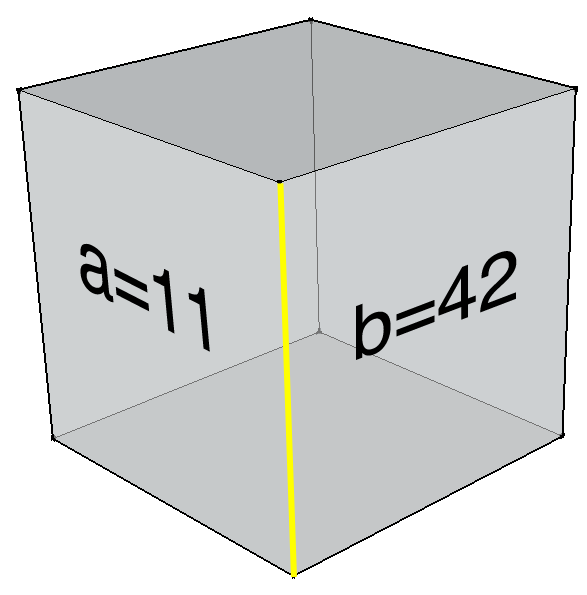
\includegraphics[width=0.32\textwidth]{./figures/counting_cube.png}
  \caption{Cube used to compare ratios of paths.  Yellow edge indicates ratio a/b.}
  \label{fig:unitCubes}
\end{wrapfigure}


Method:
\begin{itemize}
 \item partition space into boxes
 \item enumerate the boxes
 \item map a concrete positional trace through space onto its uniquely corresponding boxes
 \item sync time frames of box-traces to infer spatio-temporal properties
 \item using the spatio-temporal box-trace, derive properties (given elsewhere)
\end{itemize}

\emph{Selecting appropriate box size}

Different box sizes may generate very different properties.

\emph{Too small of a box} If you choose the boxes to be relatively small, the trace may show a teleport, which we define as a spatially disconnected box-trace.
If there are gaps of disconnected boxes, and two entities collide in the unaccounted for space, the violation of box-independence will not be inferred.

\emph{Too big of a box} If you choose the boxes to be relatively large, this may be too rough of an over approximation.
For an extreme example, an entity never registers "leaving home" if its initial box is the size of the given dimensions.
Sometimes large over-approximations are desired, such as if you only want to examine the movements across two ``hemispheres" of an entity's space.
